\documentclass[10pt,twocolumn,letterpaper]{article}

\usepackage{cvpr}
\usepackage{times}
\usepackage{graphicx}
\usepackage{amsmath}
\usepackage{amssymb}
\usepackage{listings}
\usepackage{xcolor}
\usepackage[breaklinks=true,bookmarks=false]{hyperref}

\cvprfinalcopy
\setcounter{page}{1}

\lstset{
  basicstyle=\ttfamily\scriptsize,
  breaklines=true,
  frame=single,
  columns=fullflexible,
  keepspaces=true,
  xleftmargin=2pt,
  xrightmargin=2pt
}

\begin{document}

\title{Feature-based Image Matching and Automatic Panorama Construction\\{\large Submission packet}}

\author{
Shadrack Bentil\\
MSc Computer Science\\
University of Ghana, Legon\\
{\tt\small sbentil005@st.ug.edu.gh}
}

\maketitle

\begin{abstract}
This packet summarises a classical OpenCV panorama pipeline (detect $\rightarrow$ describe $\rightarrow$ match $\rightarrow$ RANSAC $\rightarrow$ homography $\rightarrow$ warp $\rightarrow$ stitch), with source excerpts, experiment figures, and screenshots of the interactive app. The full CVPR-formatted report, code, and data live in the public repository. The live demonstration is hosted on Streamlit Community Cloud.
\end{abstract}

\section{Where to find the work}

\begin{itemize}
\item \textbf{Live app:} \url{https://feature-based-panorama.streamlit.app/}
\item \textbf{Source (public):} \url{https://github.com/qbentil/feature-based-panorama}
\item \textbf{Full report PDF} in the repo: \texttt{report/feature\_based\_panorama.pdf} (also embedded on the app's Project report tab)
\end{itemize}

The repository contains the pipeline under \texttt{src/}, the Streamlit walkthrough under \texttt{app\_pages/}, Wikimedia Commons campus photographs (Balme Library, Dance Department, Night Market, Commonwealth Hall) with licences in \texttt{data/ATTRIBUTION.md}, and experiment tables in \texttt{report/results/}.

The implementation does \textbf{not} call \texttt{cv2.Stitcher}, YOLO, or any pretrained recogniser.

\section{App walkthrough}

Six tabs: How it works, Build a panorama, Compare detectors, Robustness lab, Saved results, Project report.

\begin{figure*}[t]
\centering
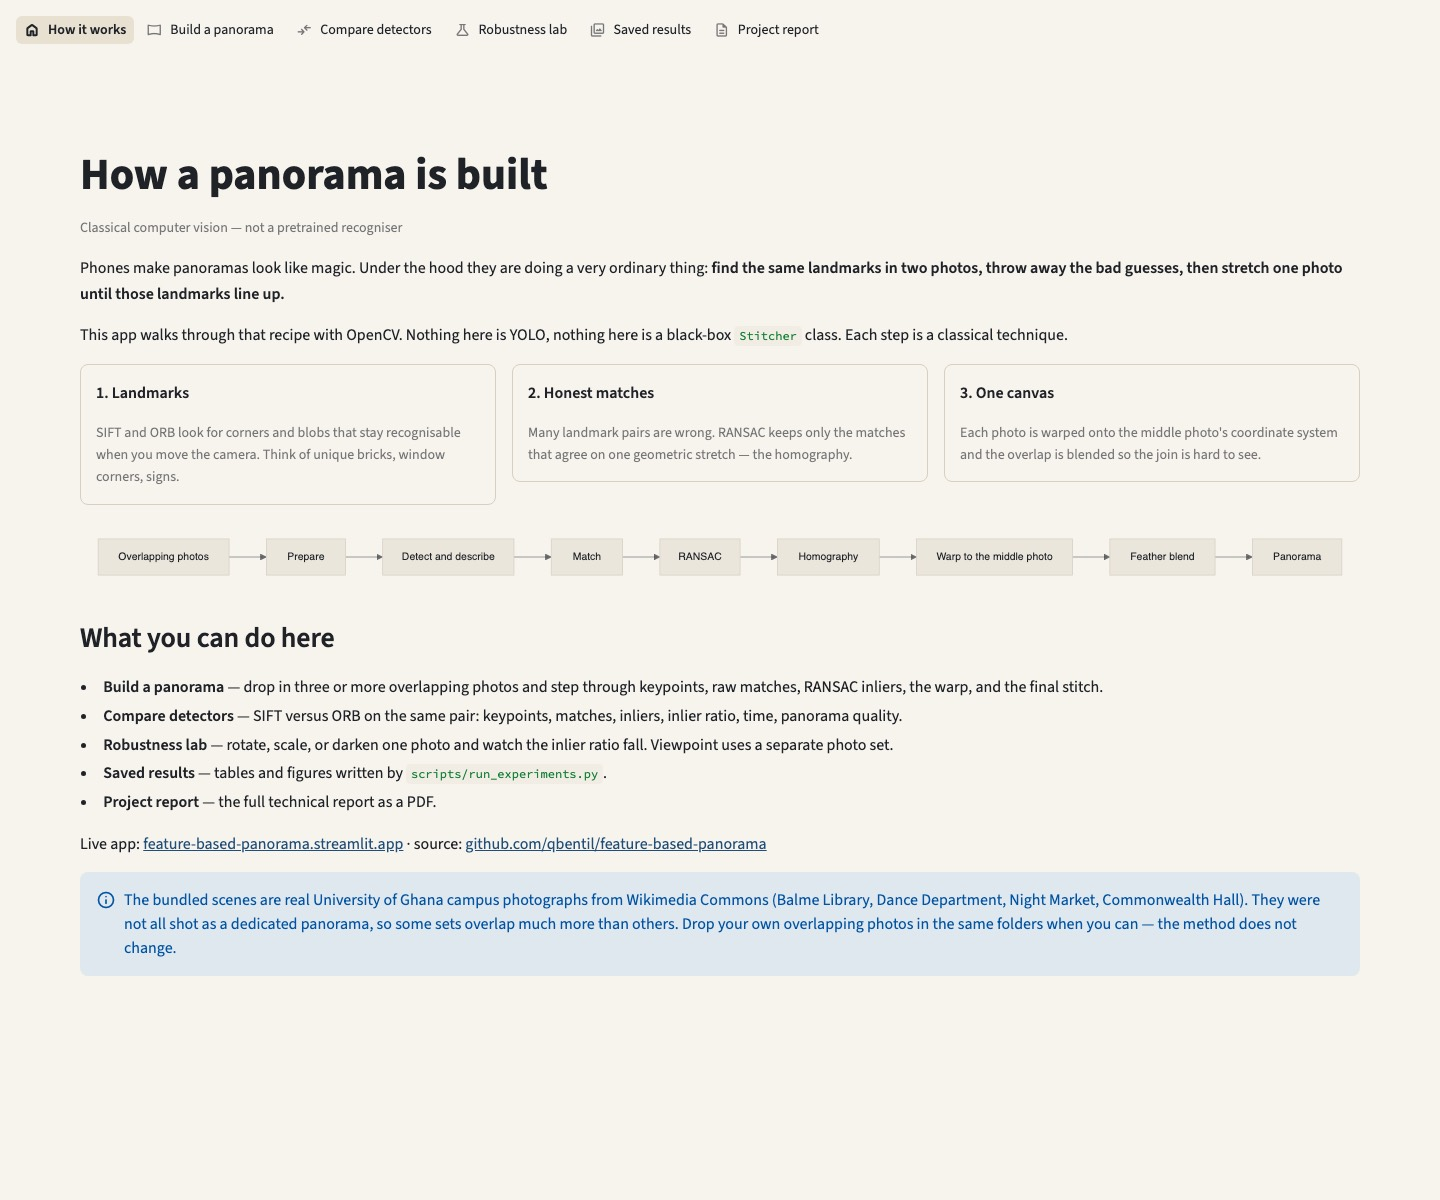
\includegraphics[width=0.48\linewidth]{submission_shots/home.jpg}\hfill
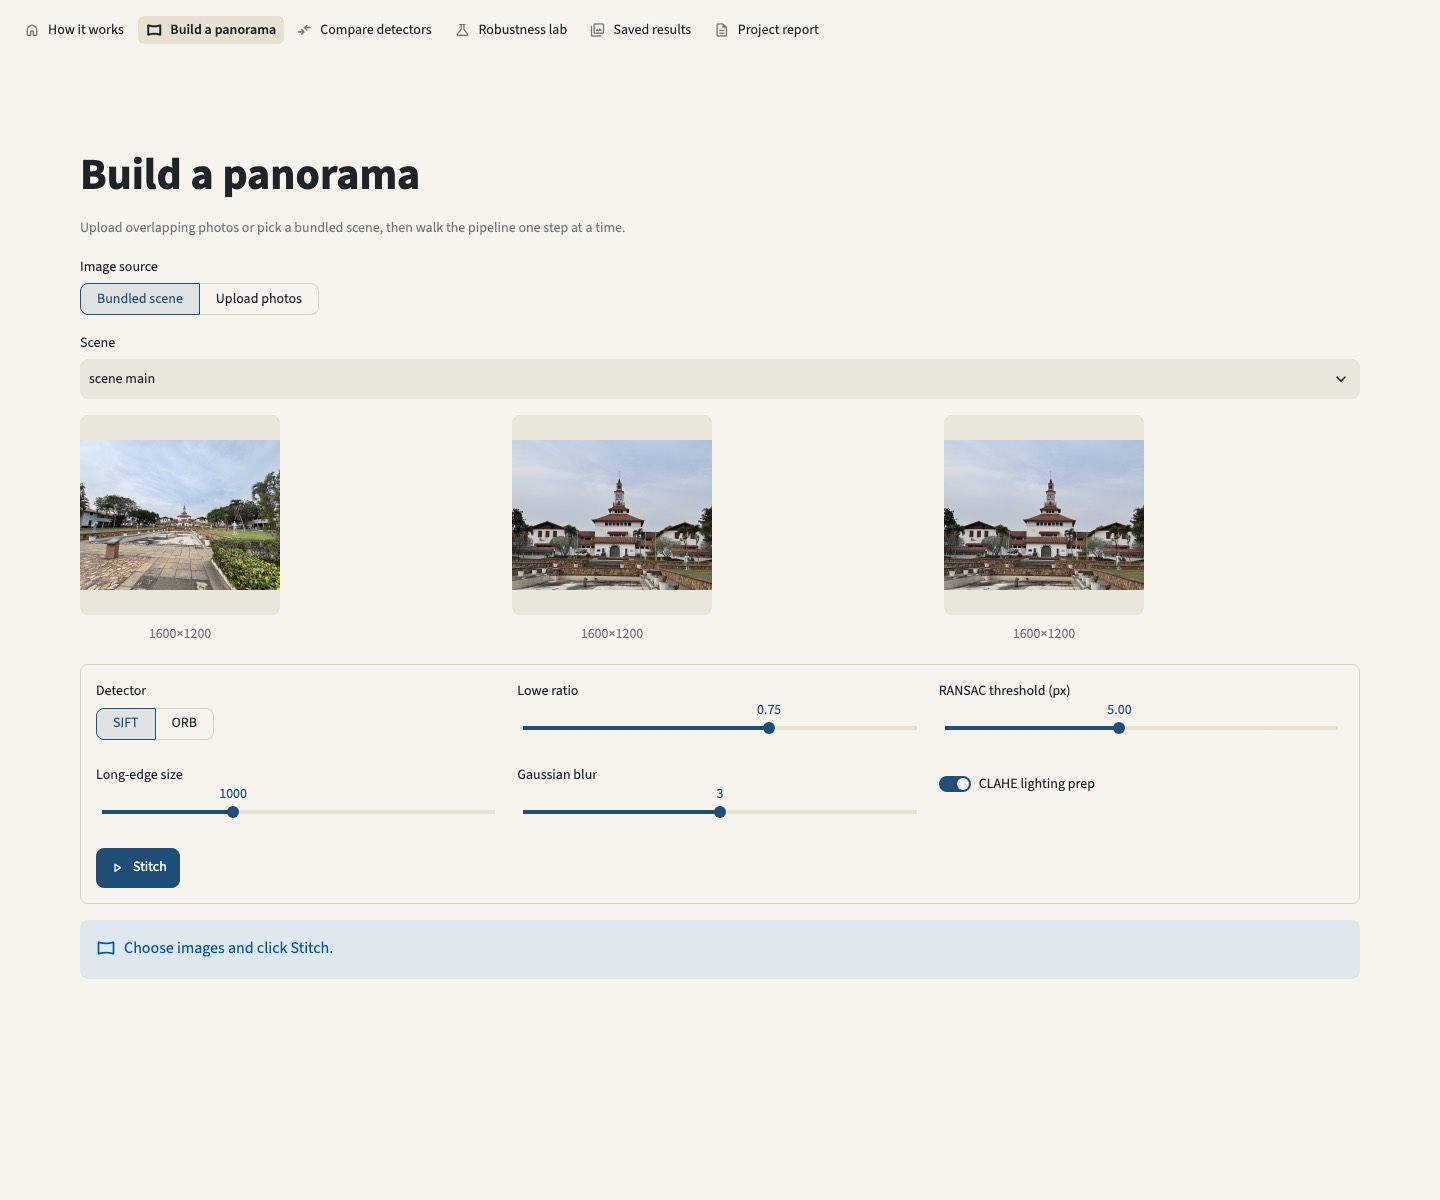
\includegraphics[width=0.48\linewidth]{submission_shots/stitch.jpg}
\caption{Left: How it works (pipeline explanation). Right: Build a panorama with bundled Balme Library views, SIFT, Lowe ratio 0.75, RANSAC 5\,px.}
\label{fig:ui1}
\end{figure*}

\begin{figure*}[t]
\centering
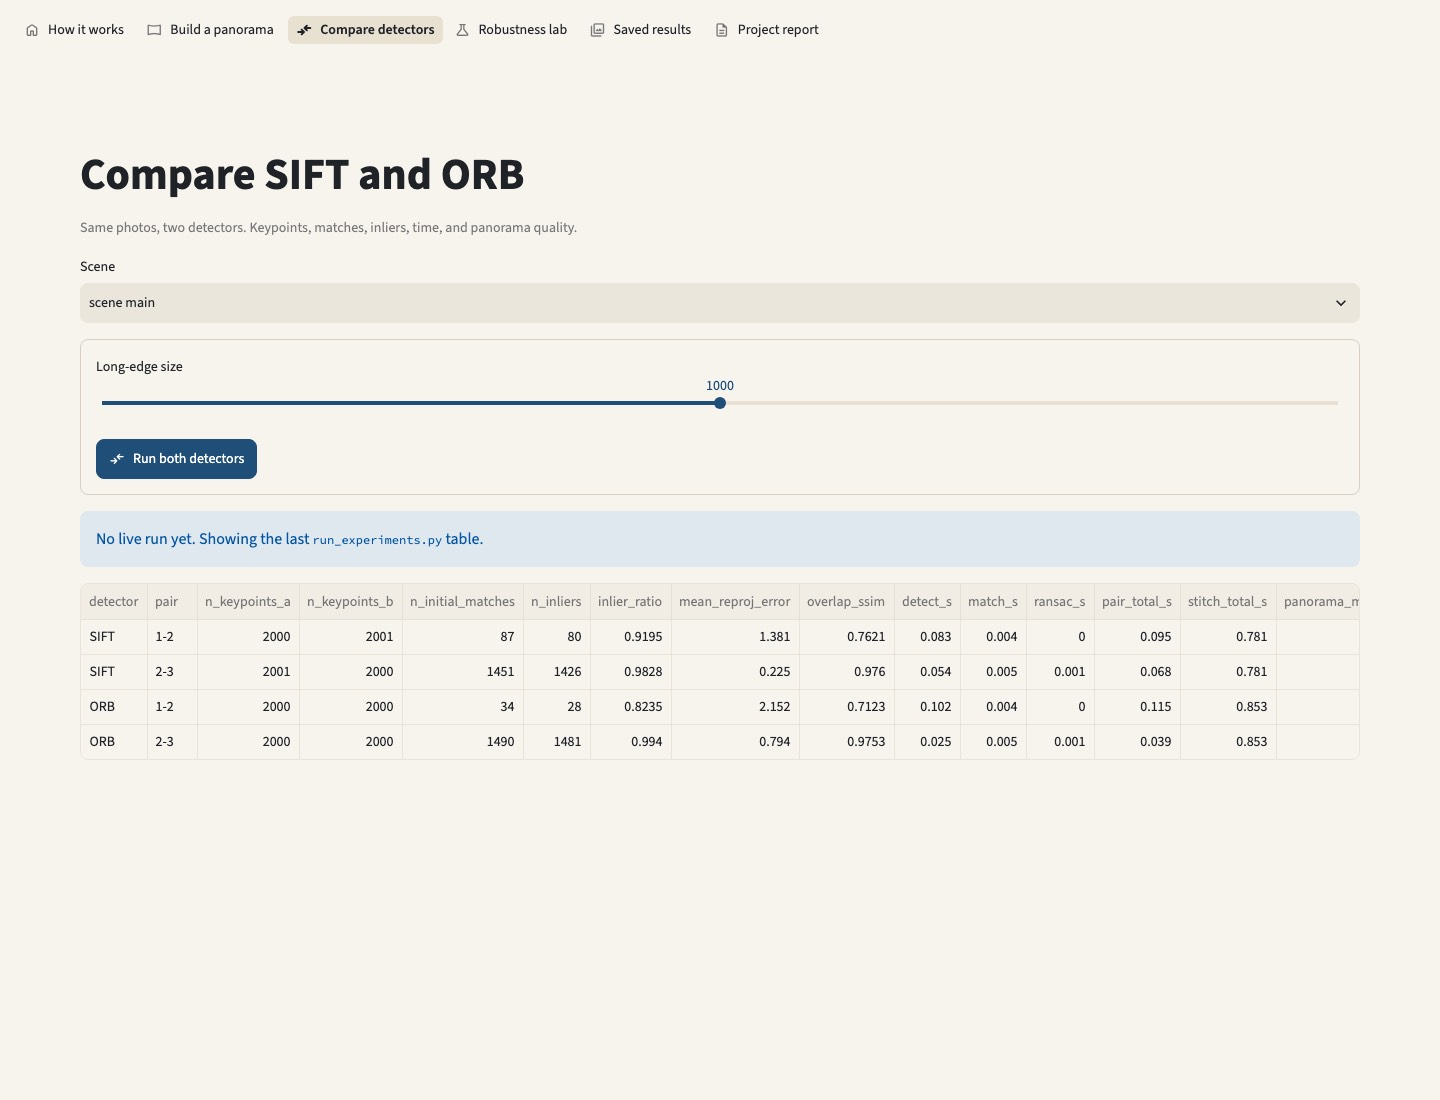
\includegraphics[width=0.48\linewidth]{submission_shots/compare.jpg}\hfill
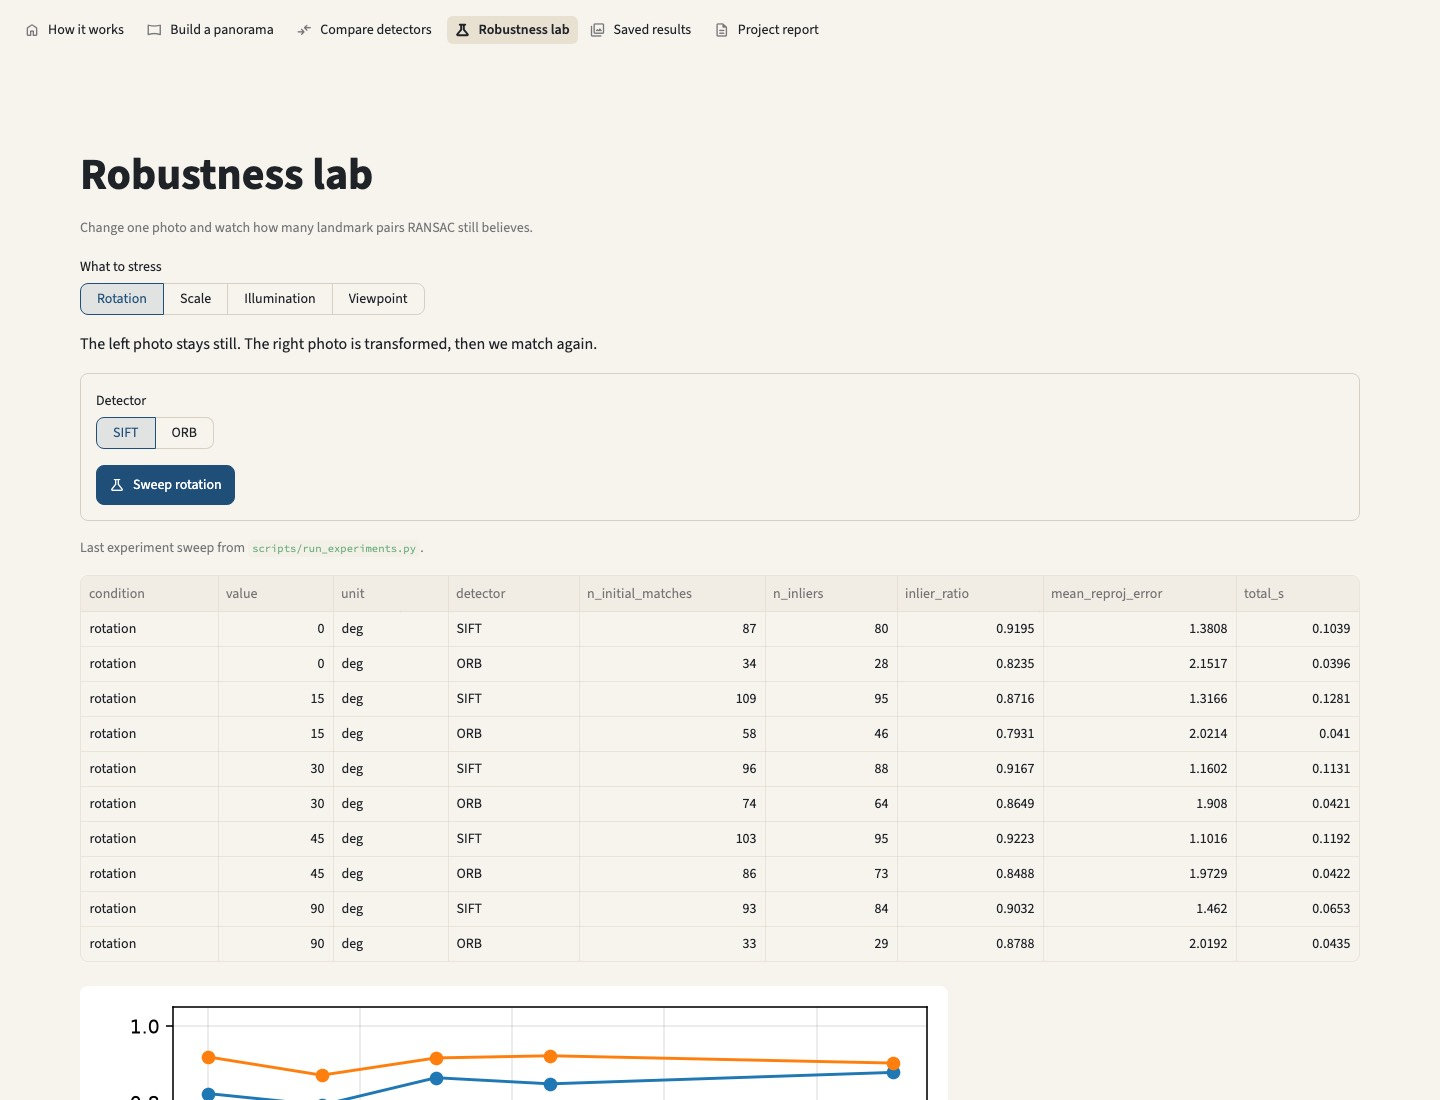
\includegraphics[width=0.48\linewidth]{submission_shots/robustness.jpg}
\caption{Left: Compare detectors (SIFT vs ORB table). Right: Robustness lab (rotation sweep).}
\label{fig:ui2}
\end{figure*}

\begin{figure}[t]
\centering
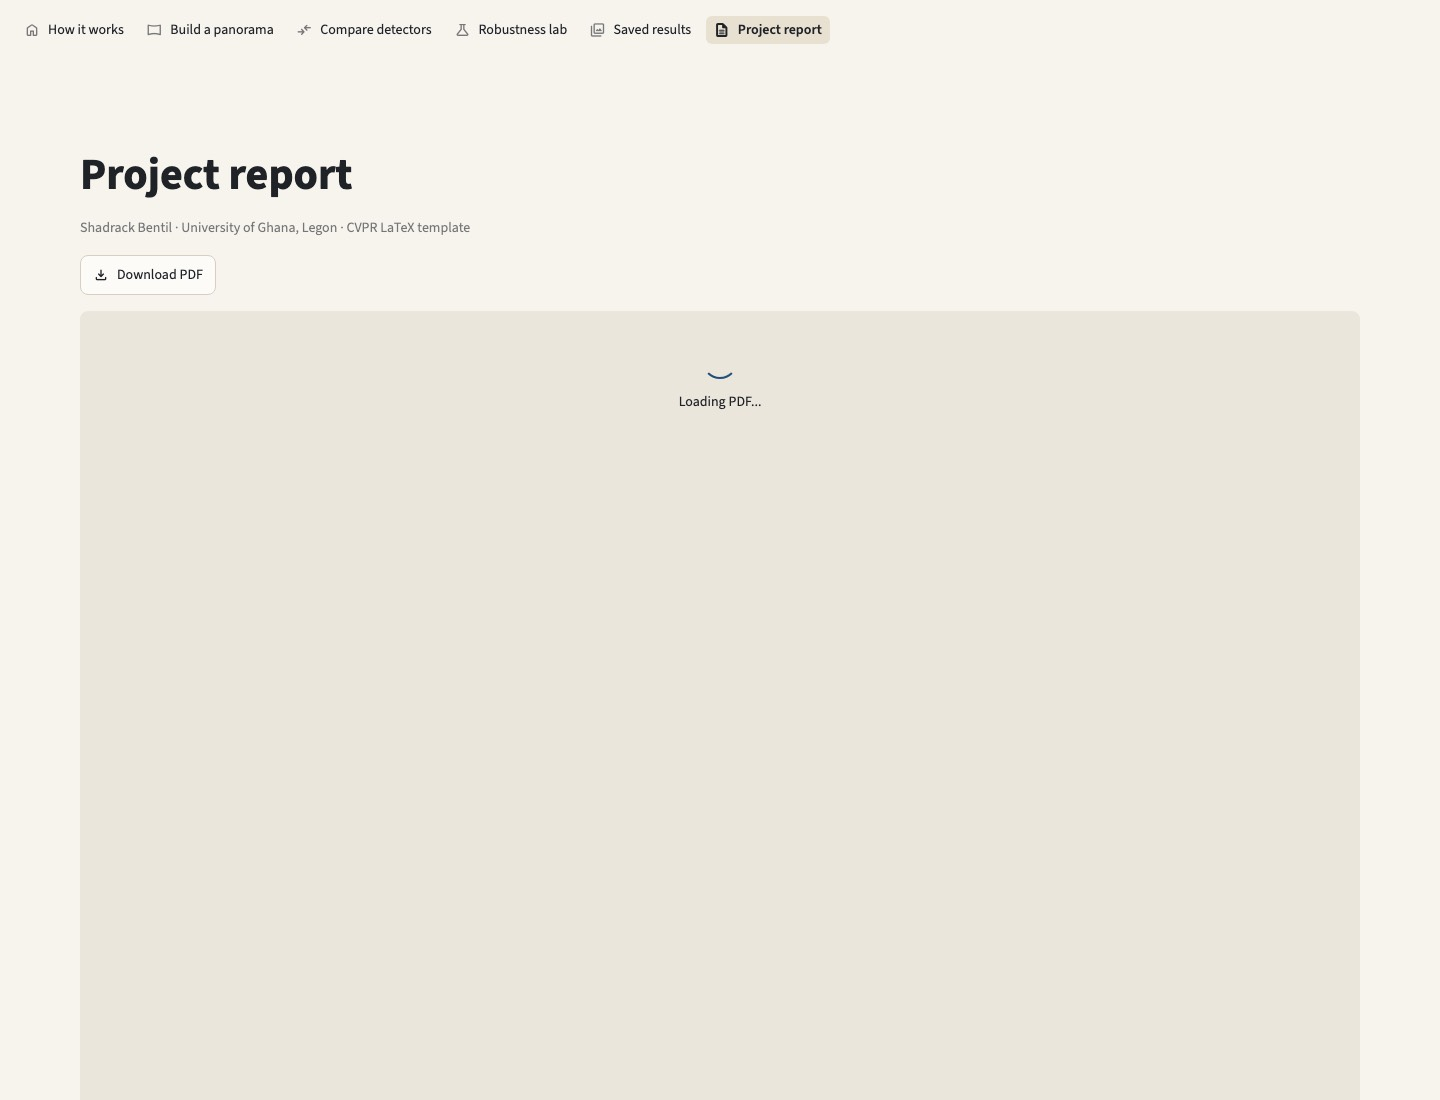
\includegraphics[width=0.98\linewidth]{submission_shots/report.jpg}
\caption{Project report tab: download and embed the full CVPR PDF.}
\label{fig:uireport}
\end{figure}

\section{Method (source excerpts)}

Shared code is in \texttt{src/}. The app never duplicates the geometry: both the UI and \texttt{scripts/run\_experiments.py} call \texttt{match\_pair} / \texttt{stitch\_images}.

\paragraph{Detect and describe.}
SIFT and ORB, capped at 2000 keypoints.

\begin{lstlisting}[language=Python]
def create_detector(name, n_features=2000):
    key = name.strip().upper()
    if key == "SIFT":
        return cv2.SIFT_create(nfeatures=n_features)
    if key == "ORB":
        return cv2.ORB_create(nfeatures=n_features)
\end{lstlisting}

\paragraph{Match.}
Brute-force $k$NN ($k{=}2$) and Lowe's ratio test. SIFT uses $L_2$; ORB uses Hamming.

\begin{lstlisting}[language=Python]
knn = matcher.knnMatch(descriptors_a, descriptors_b, k=2)
for best, second in knn:
    if best.distance < ratio * second.distance:
        good.append(best)
\end{lstlisting}

\paragraph{RANSAC homography.}
\texttt{cv2.findHomography} with a 5\,px threshold. Pairwise maps are composed into the \emph{middle} image's frame.

\begin{lstlisting}[language=Python]
H, mask = cv2.findHomography(
    pts_src, pts_dst, method=cv2.RANSAC,
    ransacReprojThreshold=ransac_thresh)
\end{lstlisting}

\paragraph{Stitch.}
\texttt{warpPerspective} plus distance-transform feather blending. Metrics: inlier ratio, mean reprojection error, overlap SSIM.

\section{Evidence}

Primary scene: three Balme Library photographs (Wikimedia Commons, CC~BY~4.0). Pair 2--3 is a near-duplicate facade (SIFT 1426 inliers, SSIM $0.976$). Pair 1--2 is courtyard-to-facade (80 inliers, SSIM $0.762$, reprojection $1.38$\,px). Mean inlier ratio: SIFT $0.951$, ORB $0.909$. Full stitch about $0.8$\,s. Gain $0.35$ illumination leaves SIFT with zero inliers. Dance Department viewpoint frames barely overlap.

\begin{figure*}[t]
\centering
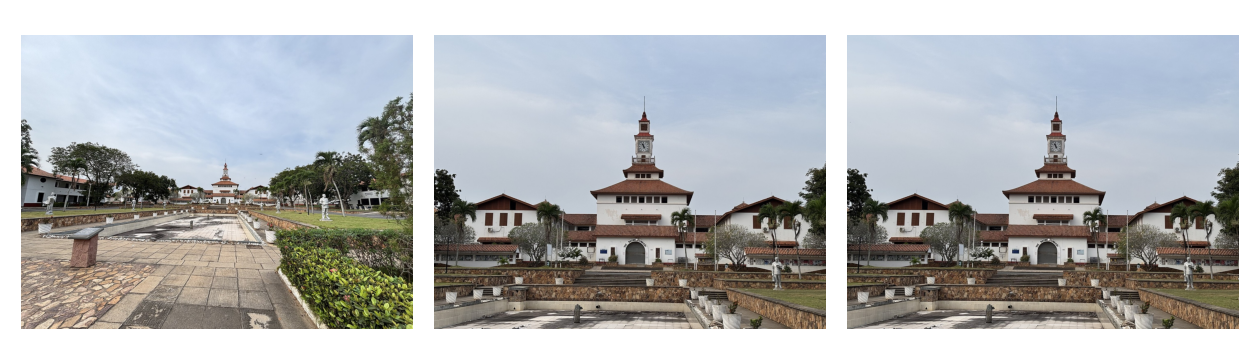
\includegraphics[width=0.98\linewidth]{figures/input_scene_main.png}
\caption{Input views for the primary stitch (Balme Library).}
\label{fig:input}
\end{figure*}

\begin{figure*}[t]
\centering
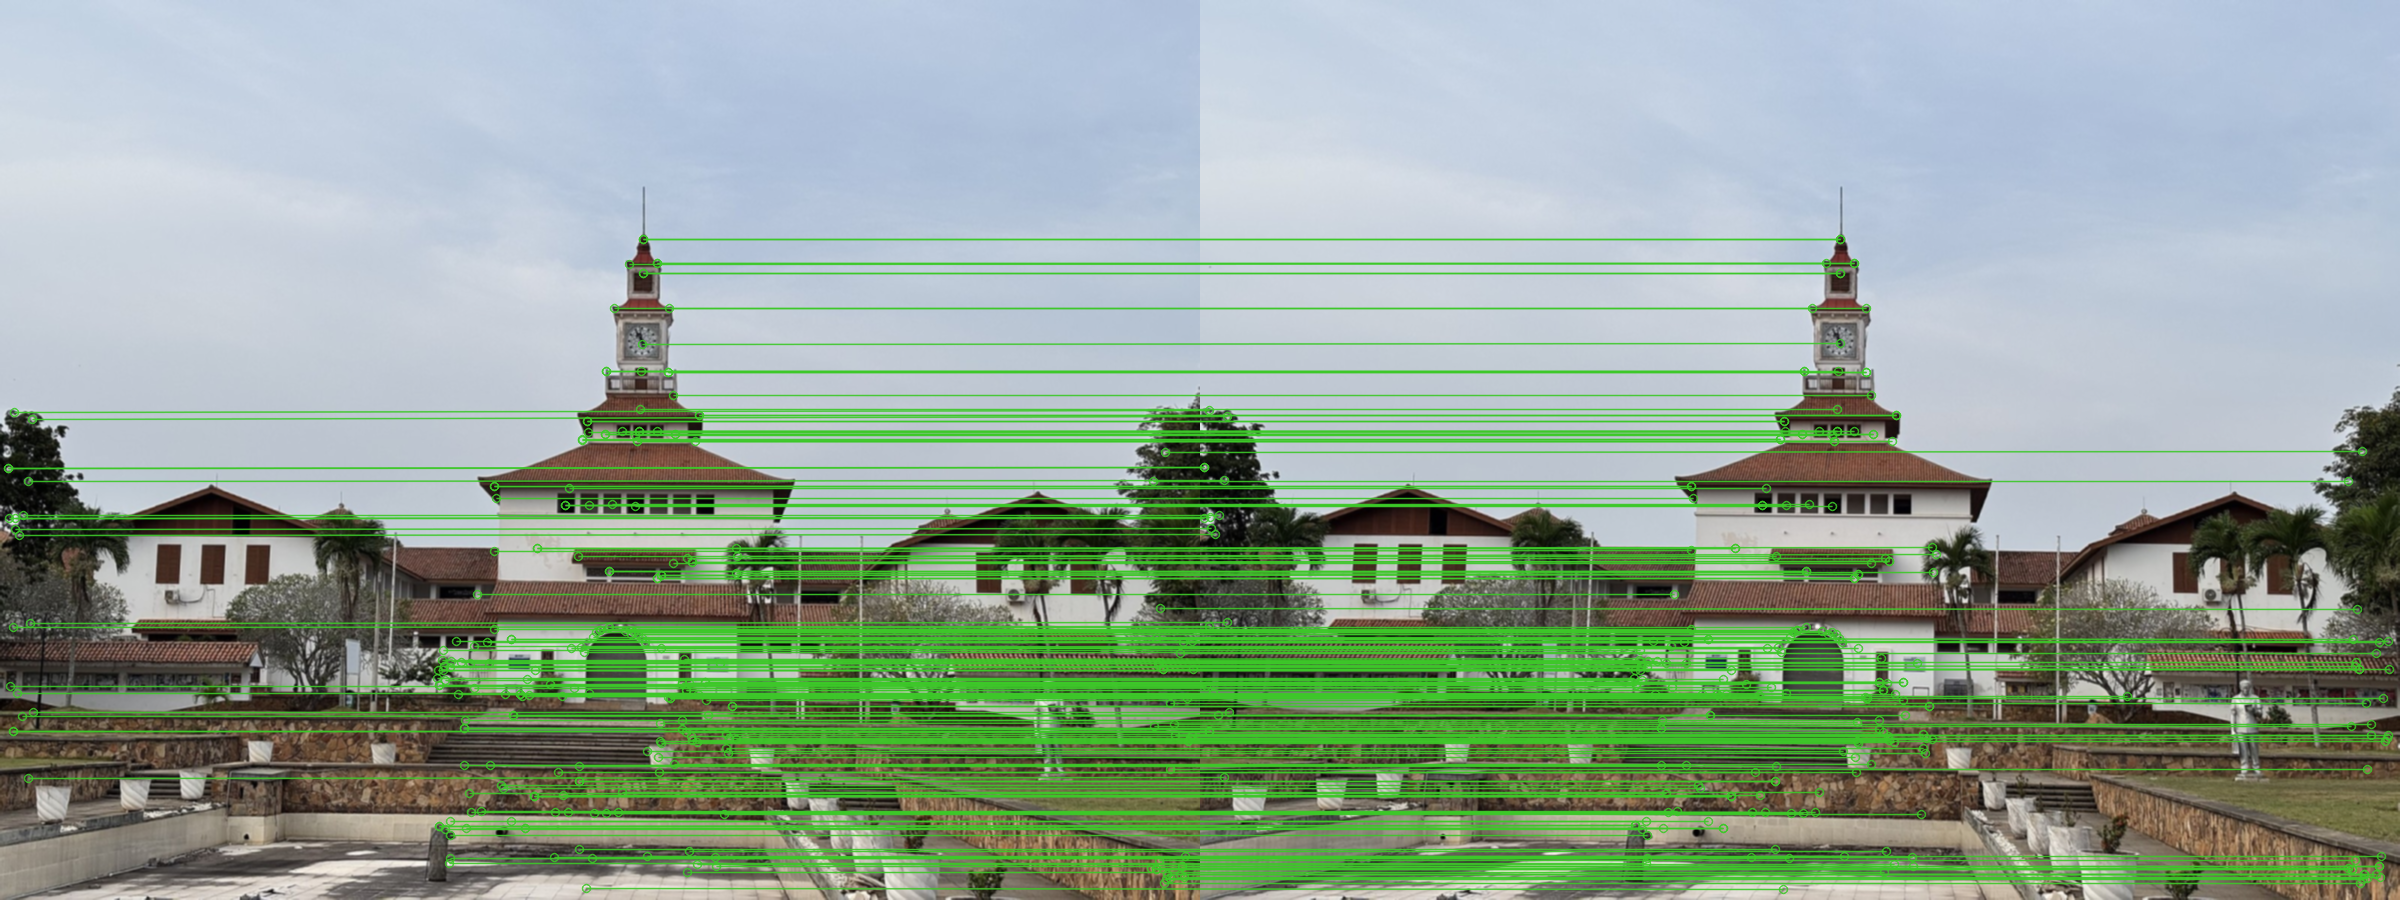
\includegraphics[width=0.48\linewidth]{figures/matches_after_sift.png}\hfill
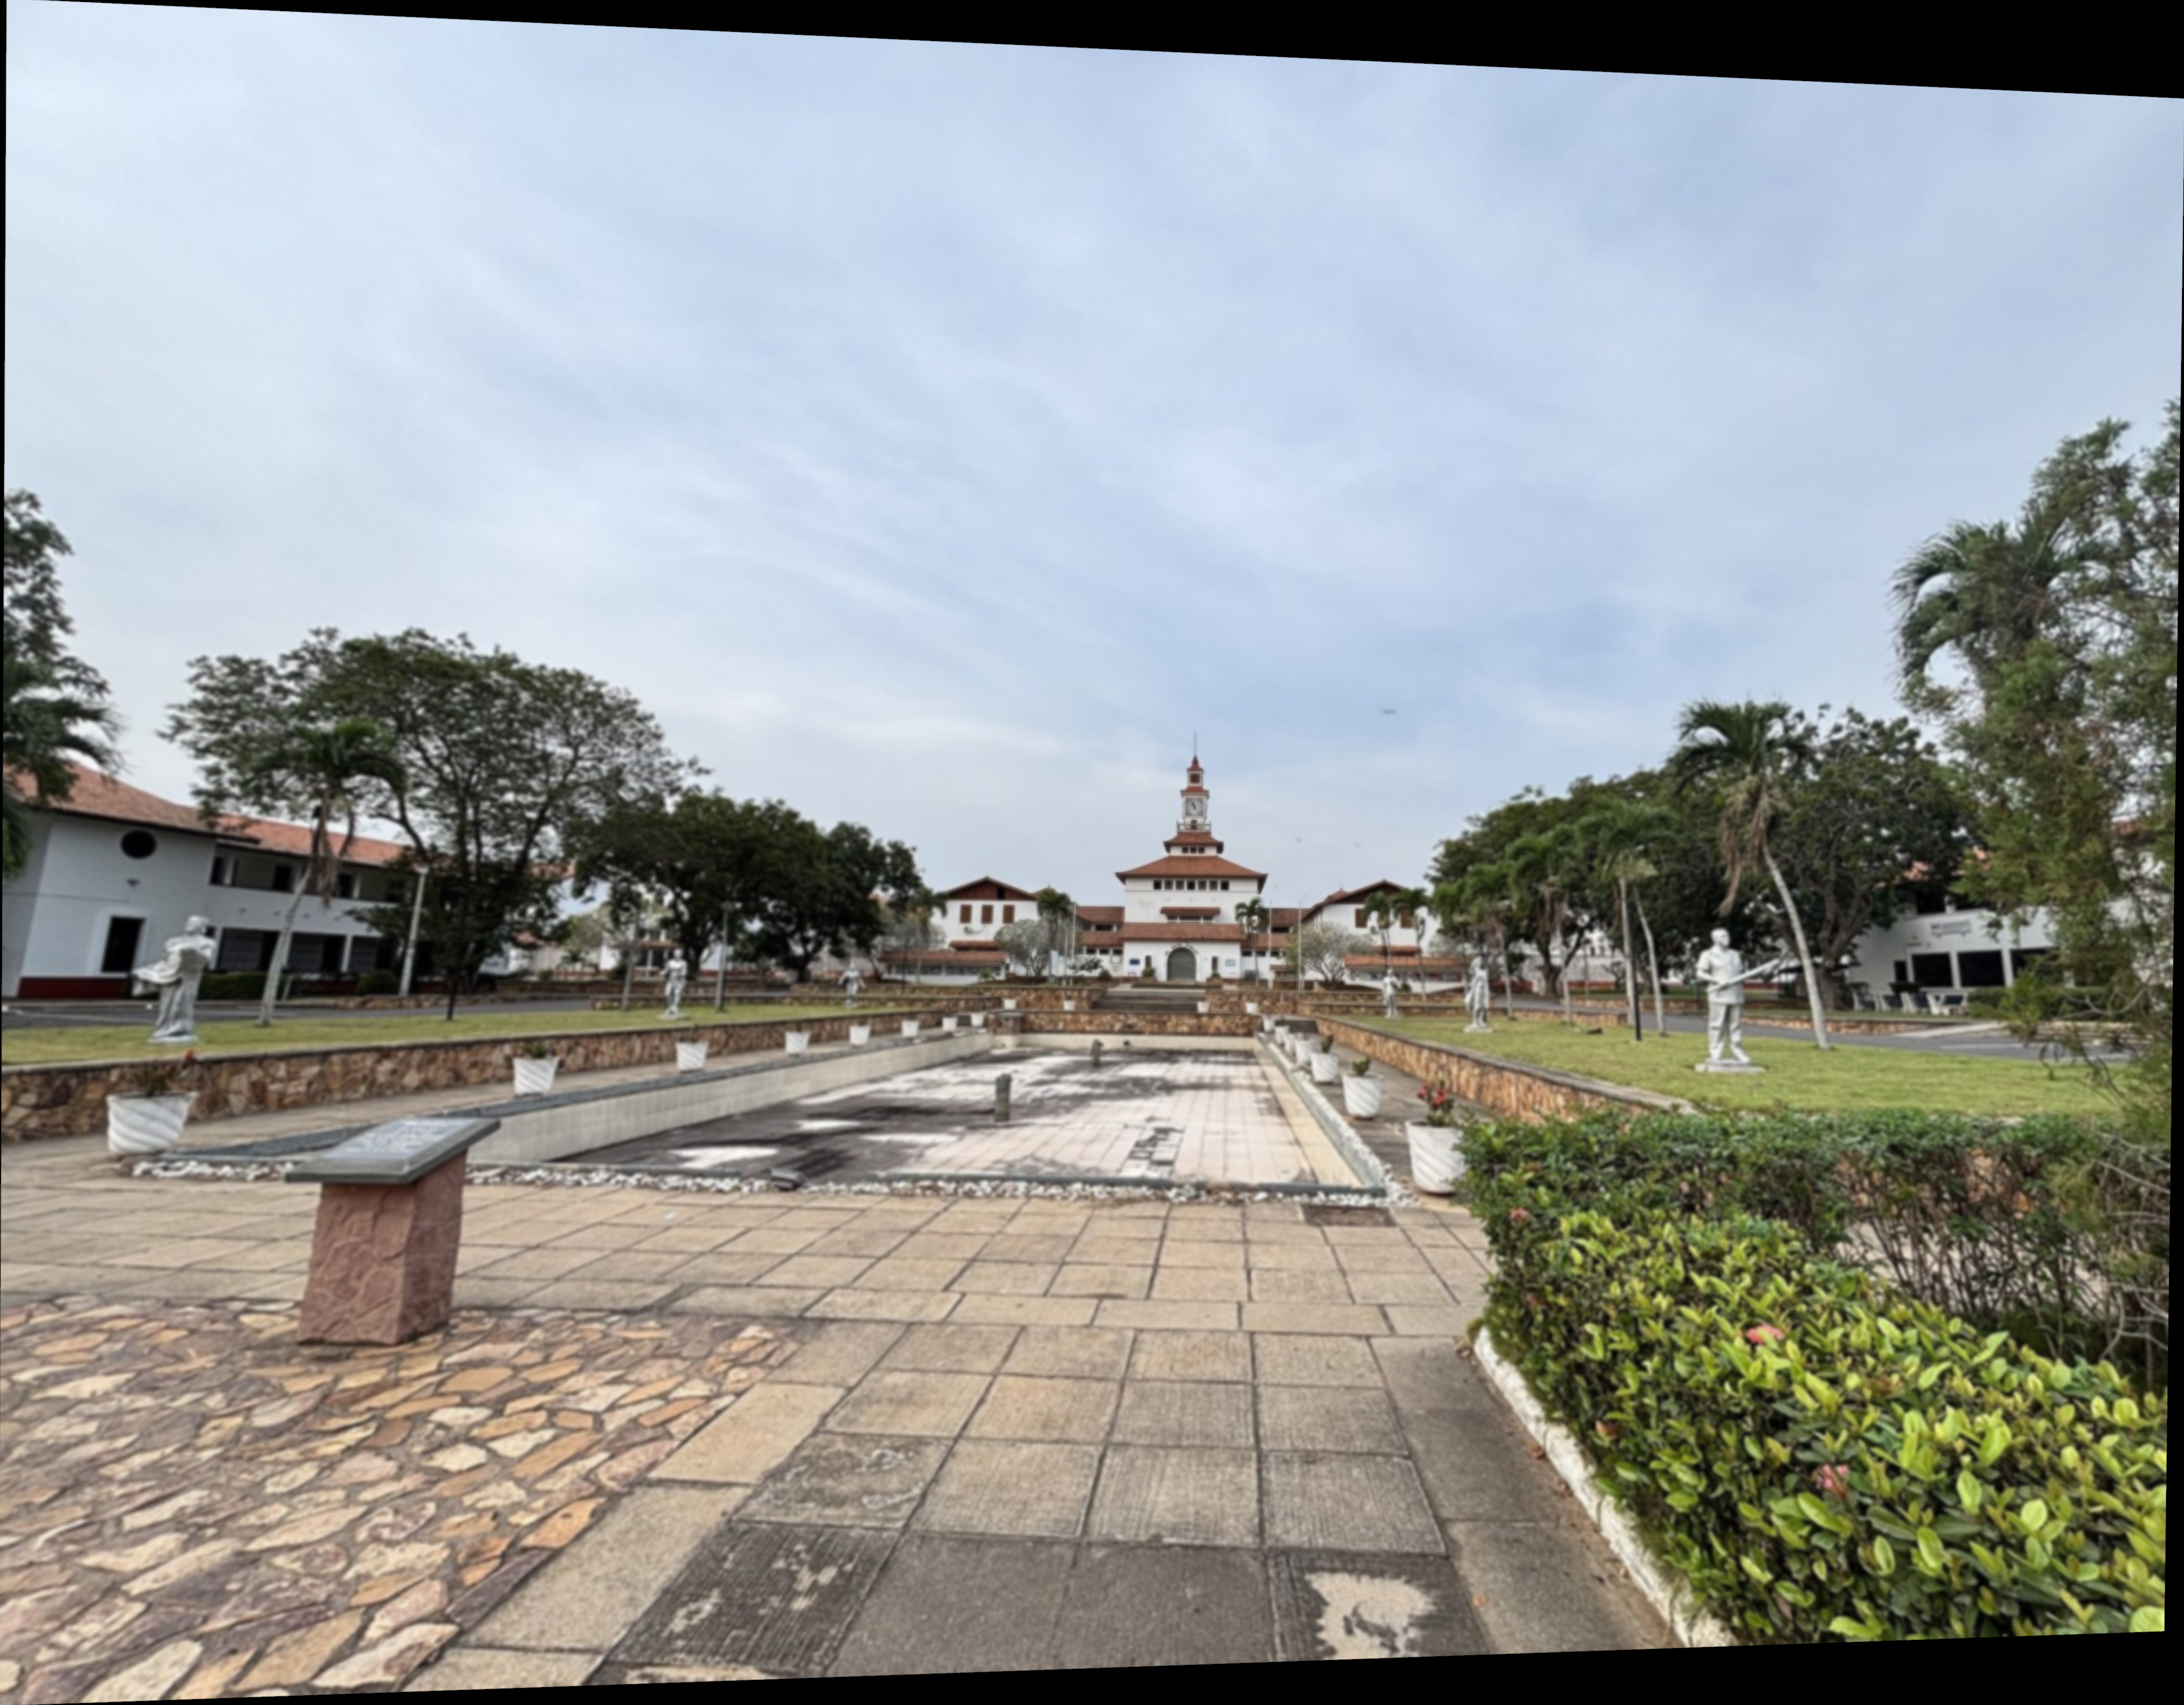
\includegraphics[width=0.48\linewidth]{figures/panorama_sift.png}
\caption{Left: SIFT inliers after RANSAC. Right: stitched panorama.}
\label{fig:pano}
\end{figure*}

\begin{figure*}[t]
\centering
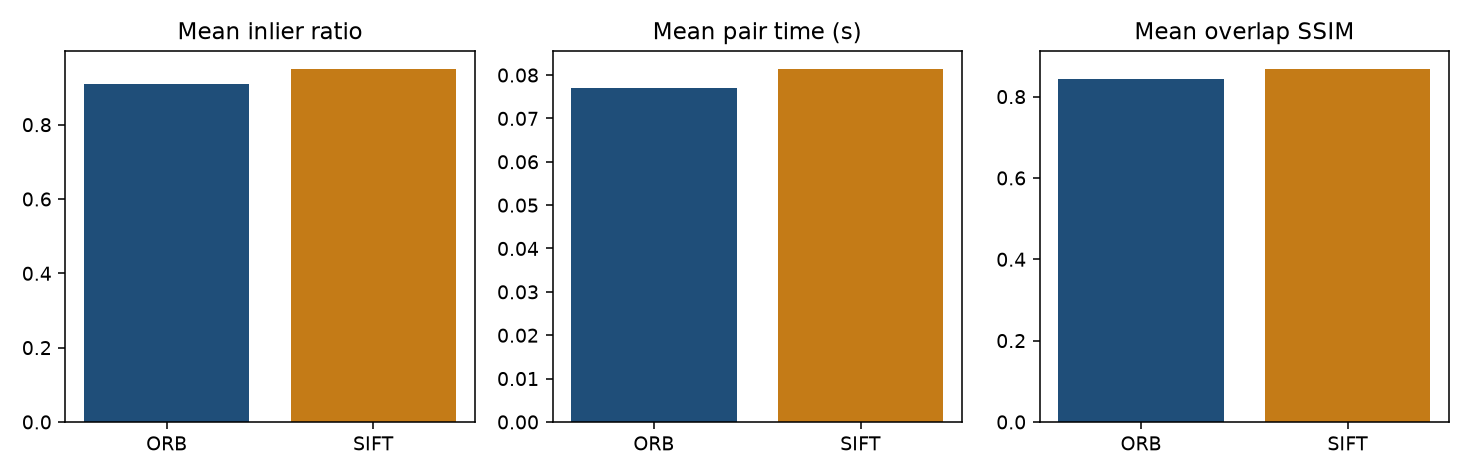
\includegraphics[width=0.48\linewidth]{figures/detector_comparison.png}\hfill
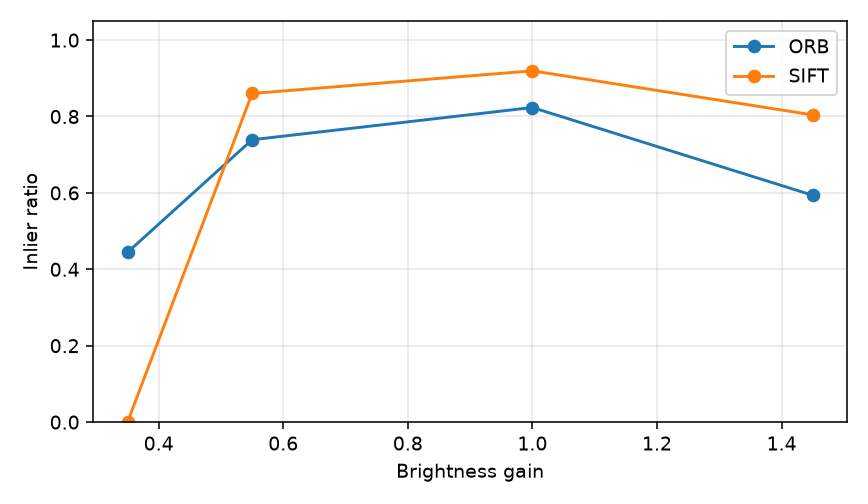
\includegraphics[width=0.48\linewidth]{figures/robustness_illumination.png}
\caption{Left: SIFT vs ORB summary. Right: illumination sweep (inlier ratio vs brightness gain).}
\label{fig:bars}
\end{figure*}

\begin{table}[t]
\centering
\setlength{\tabcolsep}{2.4pt}
{\scriptsize
\begin{tabular}{|l|c|c|c|c|c|}
\hline
Det. & Pair & Init. & Inliers & Ratio & SSIM \\
\hline\hline
SIFT & 1--2 & 87 & 80 & 0.920 & 0.762 \\
SIFT & 2--3 & 1451 & 1426 & 0.983 & 0.976 \\
ORB & 1--2 & 34 & 28 & 0.824 & 0.712 \\
ORB & 2--3 & 1490 & 1481 & 0.994 & 0.975 \\
\hline
\end{tabular}
}
\caption{Detector comparison on Balme Library consecutive pairs.}
\label{tab:det}
\end{table}

\section{How to reproduce}

\begin{lstlisting}[language=bash]
pip install -r requirements.txt
python scripts/run_experiments.py
streamlit run streamlit_app.py
\end{lstlisting}

Or open the live URL above. Bundled photos can be replaced with phone captures (30--50\% overlap, left to right) in \texttt{data/scenes/}.

\end{document}
